\documentclass[../main.tex]{subfiles}

\pagestyle{main}
\renewcommand{\sectionmark}[1]{\markboth{#1\ \thesection}{}}

\begin{document}




\section{Script}
\subsection{Journal}
\stepcounter{theorem}
\begin{definition}\label{dfn:1.2}\marginnote{10/1:}
    Two sets $A$ and $B$ are \textbf{equal} if they contain precisely the same elements, that is, $x\in A$ if and only if $x\in B$. When $A$ and $B$ are equal, we denote this by $A=B$.
\end{definition}

\begin{definition}\label{dfn:1.3}
    A set $A$ is a \textbf{subset} of a set $B$ if every element of $A$ is also an element of $B$, that is, if $x\in A$, then $x\in B$. When $A$ is a subset of $B$, we denote this by $A\subset B$. If $A\subset B$ but $A\neq B$, we say that $A$ is a \textbf{proper subset} of $B$, and we denote this by $A\subsetneq B$.
\end{definition}

\begin{exercise}\label{exr:1.4}\marginnote{10/6:}
    Let $A=\{1,\{2\}\}$. Is $1\in A$? Is $2\in A$? Is $\{1\}\subset A$? Is $\{2\}\subset A$? Is $1\subset A$? Is $\{1\}\in A$? Is $\{2\}\in A$? Is $\{\{2\}\}\subset A$? Explain.
    \begin{proof}
        We list affirmative or negative answers and short explanations.\\[3pt]
        Yes, $1\in A$.\\
        No, $2\notin A$, but $\{2\}\in A$.\\
        Yes, $\{1\}\subset A$ since 1 is the only element of $\{1\}$ and $1\in A$ (as previously established).\\
        No, $\{2\}\not\subset A$ since $2\in\{2\}$ but $2\notin A$ (as previously established).\\
        No, $1\not\subset A$ since 1 is not a set.\\
        No, $\{1\}\notin A$, but $1\in A$ and $\{1\}\subset A$ as previously established.\\
        Yes, $\{2\}\in A$.\\
        Yes, $\{\{2\}\}\subset A$ since $\{2\}$ is the only element of $\{\{2\}\}$ and $\{2\}\in A$ (as previously established).
    \end{proof}
\end{exercise}

\begin{definition}\label{dfn:1.5}\marginnote{10/1:}
    Let $A$ and $B$ be two sets. The \textbf{union} of $A$ and $B$ is the set
    \begin{equation*}
        A\cup B = \{x\mid x\in A\text{ or }x\in B\}
    \end{equation*}
\end{definition}

\begin{definition}\label{dfn:1.6}
    Let $A$ and $B$ be two sets. The \textbf{intersection} of $A$ and $B$ is the set
    \begin{equation*}
        A\cap B = \{x\mid x\in A\text{ and }x\in B\}
    \end{equation*}
\end{definition}

\stepcounter{theorem}

\begin{definition}\label{dfn:1.8}
    The \textbf{empty set} is the set with no elements, and it is denoted $\emptyset$. That is, no matter what $x$ is, we have $x\in\emptyset$.
\end{definition}

\begin{definition}\label{dfn:1.9}
    Two sets $A$ and $B$ are \textbf{disjoint} if $A\cap B=\emptyset$.
\end{definition}

\begin{exercise}\label{exr:1.10}\marginnote{10/6:}
    Show that if $A$ is any set, then $\emptyset\subset A$.
    \begin{proof}
        Suppose for the sake of contradiction that there exists a set $A$ such that $\emptyset\not\subset A$. Then by Definition \ref{dfn:1.3}, not every element of $\emptyset$ is also an element of $A$, i.e., there exists an element $x\in\emptyset$ such that $x\notin A$. But by Definition \ref{dfn:1.8}, $x$ (like all other objects) cannot be an element of $\emptyset$, a contradiction. Therefore, $\emptyset\subset A$ for all sets $A$.
    \end{proof}
\end{exercise}

\begin{definition}\label{dfn:1.11}\marginnote{10/1:}
    Let $A$ and $B$ be two sets. The \textbf{difference} of $B$ from $A$ is the set
    \begin{equation*}
        A\setminus B = \{x\in A\mid x\notin B\}
    \end{equation*}
    The set $A\setminus B$ is also called the \textbf{complement} of $B$ relative to $A$. When the set $A$ is clear from the context, this set is sometimes denoted $B^c$, but we will try to avoid this imprecise formulation and use it only with warning.
\end{definition}

\begin{theorem}\label{trm:1.12}
    Let $X$ be a set, and let $A,B\subset X$. Then
    \begin{enumerate}[label={\alph*\textup{)}}]
        \item $X\setminus(A\cup B)=(X\setminus A)\cap(X\setminus B)$
        \item $X\setminus(A\cap B)=(X\setminus A)\cup(X\setminus B)$
    \end{enumerate}
    \begin{proof}[Proof of a]
        To prove that $X\setminus(A\cup B)=(X\setminus A)\cap(X\setminus B)$, Definition \ref{dfn:1.2} tells us that it will suffice to prove that $x\in X\setminus(A\cup B)$ if and only if $x\in (X\setminus A)\cap(X\setminus B)$, i.e., that if $x\in X\setminus(A\cup B)$, then $x\in (X\setminus A)\cap(X\setminus B)$ and if $x\in (X\setminus A)\cap(X\setminus B)$, then $x\in X\setminus(A\cup B)$. To begin, let $x\in X\setminus(A\cup B)$. By Definition \ref{dfn:1.11}, $x\in X$ and $x\notin A\cup B$. By Definition \ref{dfn:1.5}, it follows that $x\notin A$ and $x\notin B$. Since we know that $x\in X$ and $x\notin A$, Definition \ref{dfn:1.11} tells us that $x\in X\setminus A$. Similarly, $x\in X\setminus B$. Since $x\in X\setminus A$ and $x\in X\setminus B$, we have by Definition \ref{dfn:1.6} that $x\in(X\setminus A)\cap(X\setminus B)$, as desired. The proof of the other implication is the preceding proof "in reverse." For clarity, let $x\in(X\setminus A)\cap(X\setminus B)$. By Definition \ref{dfn:1.6}, $x\in X\setminus A$ and $x\in X\setminus B$. By consecutive applications of Definition \ref{dfn:1.11}, $x\in X$, $x\notin A$, and $x\notin B$. Since $x\notin A$ and $x\notin B$, Definition \ref{dfn:1.5} reveals that $x\notin A\cup B$. But as previously established, $x\in X$, so Definition \ref{dfn:1.11} tells us that $x\in X\setminus(A\cup B)$.
    \end{proof}
    \begin{proof}[Proof of b]
        To prove that $X\setminus(A\cap B)=(X\setminus A)\cup(X\setminus B)$, Definition \ref{dfn:1.2} tells us that it will suffice to prove that $x\in X\setminus(A\cap B)$ if and only if $x\in (X\setminus A)\cup(X\setminus B)$. To begin, let $x\in X\setminus(A\cap B)$. By Definition \ref{dfn:1.11}, $x\in X$ and $x\notin A\cap B$. By Definition \ref{dfn:1.6}, it follows that $x\notin A$ or $x\notin B$. We divide into two cases. If $x\notin A$, then since we know that $x\in X$, Definition \ref{dfn:1.11} tells us that $x\in X\setminus A$. It naturally follows that $x\in(X\setminus A)\cup(X\setminus B)$, since $x$ need only be an element of one of the two unionized sets (see Definition \ref{dfn:1.5}). The proof is symmetric if $x\notin B$. Now let $x\in(X\setminus A)\cup(X\setminus B)$. By Definition \ref{dfn:1.5}, $x\in X\setminus A$ or $x\in X\setminus B$. Once again, we divide into two cases. If $x\in X\setminus A$, then $x\in X$ and $x\notin A$ by Definition \ref{dfn:1.11}. Consequently, by Definition \ref{dfn:1.6}, $x\notin A\cap B$. Therefore, $x\in X\setminus(A\cap B)$ by Defintion \ref{dfn:1.11}. The proof is symmetric if $x\in X\setminus B$.
    \end{proof}
\end{theorem}

\setcounter{theorem}{14}

\begin{definition}\label{dfn:1.15}
    Let $A$ and $B$ be two nonempty sets. The \textbf{Cartesian product} of $A$ and $B$ is the set of ordered pairs
    \begin{equation*}
        A\times B = \{(a,b)\mid a\in A\text{ and }b\in B\}
    \end{equation*}
    If $(a,b),(a',b')\in A\times B$, we say that $(a,b)$ and $(a',b')$ are \textbf{equal} if and only if $a=a'$ and $b=b'$. In this case, we write $(a,b)=(a',b')$.
\end{definition}

\begin{definition}\label{dfn:1.16}
    Let $A$ and $B$ be two nonempty sets. A \textbf{function} $f$ from $A$ to $B$ is a subset $f\subset A\times B$ such that for all $a\in A$, there exists a unique $b\in B$ satisfying $(a,b)\in f$. To express the idea that $(a,b)\in f$, we most often write $f(a)=b$. To express that $f$ is a function from $A$ to $B$ in symbols, we write $f:A\to B$.
\end{definition}

\stepcounter{theorem}

\begin{definition}\label{dfn:1.18}
    Let $f:A\to B$ be a function. The \textbf{domain} of $f$ is $A$ and the \textbf{codomain} of $f$ is $B$. If $X\subset A$, then the \textbf{image} of $X$ under $f$ is the set
    \begin{equation*}
        f(X) = \{f(x)\in B\mid x\in X\}
    \end{equation*}
    If $Y\subset B$, then the \textbf{preimage} of $Y$ under $f$ is the set
    \begin{equation*}
        f^{-1}(Y) = \{a\in A\mid f(a)\in Y\}
    \end{equation*}
\end{definition}

\begin{exercise}\label{exr:1.19}
    Must $f(f^{-1}(Y))=Y$ and $f^{-1}(f(X))=X$? For each, either prove that it always holds or give a counterexample.
    \begin{proof}
        We will address each statement in turn.\par
        Consider the sets $\{1\}$ and $\{3,4\}$, and let $f:\{1\}\to\{3,4\}$ be a function defined by $f(1)=3$. Let $Y=\{4\}$ (we clearly have $Y\subset\{3,4\}$ since 4 is the only element of $Y$ and $4\in\{3,4\}$ [see Definition \ref{dfn:1.3}]). Then $f^{-1}(Y)=\{a\in\{1\}\mid f(a)\in\{4\}\}=\emptyset$ and $f(f^{-1}(Y))=\{f(x)\in\{3,4\}\mid x\in\emptyset\}=\emptyset$ by consecutive applications of Definition \ref{dfn:1.18}. Therefore, $f(f^{-1}(Y))\neq Y$ since $4\in Y$ but $4\notin f(f^{-1}(Y))$ (see Definition \ref{dfn:1.2})\footnote{Note that the reason $f(f^{-1}(Y))\neq Y$ in this case is because $f$ is not surjective.}.\par
        Similarly, consider the sets $\{1,2\}$ and $\{3\}$, and let $f:\{1,2\}\to\{3\}$ be a function defined by $f(1)=3$ and $f(2)=3$. Let $X=\{1\}$ (we clearly have $X\subset\{1,2\}$ since 1 is the only element of $X$ and $1\in\{1,2\}$ [see Definition \ref{dfn:1.3}]). Then $f(X)=\{f(x)\in\{3\}\mid x\in\{1\}\}=\{f(1)\}=\{3\}$ and $f^{-1}(f(X))=\{a\in\{1,2\}\mid f(a)\in\{3\}\}=\{1,2\}$ by consecutive applications of Definition \ref{dfn:1.18}. Therefore, $f^{-1}(f(X))\neq X$ since $2\in f^{-1}(f(X))$ but $2\notin X$ (see Definition \ref{dfn:1.2})\footnote{Note that the reason $f^{-1}(f(X))\neq X$ in this case is because $f$ is not injective.}.
    \end{proof}
\end{exercise}

\begin{definition}\label{dfn:1.20}
    A function $f:A\to B$ is \textbf{surjective} (\emph{also known as} \textbf{onto}) if for every $b\in B$, there is some $a\in A$ such that $f(a)=b$. The function $f$ is \textbf{injective} (\emph{also known as} \textbf{one-to-one}) if for all $a,a'\in A$, if $f(a)=f(a')$, then $a=a'$. The function $f$ is \textbf{bijective} (\emph{also known as} a \textbf{bijection}, a \textbf{one-to-one correspondence}) if it is surjective and injective.
\end{definition}

\begin{exercise}\label{exr:1.21}\marginnote{10/6:}
    Let $f:\N\to\N$ be defined by $f(n)=n^2$. Is $f$ injective? Is $f$ surjective?
    \begin{proof}
        $f$ is injective: Let $f(n)=f(n')$. Then $n^2=(n')^2$, implying that $n=n'$ (note that this last step is not permissible in all number systems, but it is within the naturals).\par
        $f$ is not surjective: For example, $2\in\N$ but there exists no natural number $n$ such that $f(n)=n^2=2$ (suppose for the sake of contradiction that there exists a natural number $n$ such that $n^2=2$. Since $n^2=2>1$, we know that $n<2$ (a number is less than its square if its square is greater than 1). But the only natural number less than 2 is 1, and $1^2=1\neq 2$, a contradiction).
    \end{proof}
\end{exercise}

\begin{exercise}\label{exr:1.22}
    Let $f:\N\to\N$ be defined by $f(n)=n+2$. Is $f$ injective? Is $f$ surjective?
    \begin{proof}
        $f$ is injective: Let $f(n)=f(n')$. Then $n+2=n'+2$, implying by the cancellation law for addition that $n=n'$.\par
        $f$ is not surjective: For example, $1\in\N$ but there exists no natural number $n$ such that $n+2=1$ (suppose for the sake of contradiction that there exists a natural number $n$ such that $n+2=1$. Because $1=n+2$, we know that $1>n$. But we also know that $1\leq n$ for all $n\in\N$ (as can be proven by induction), which contradicts the trichotomy).
    \end{proof}
\end{exercise}

\begin{exercise}\label{exr:1.23}
    Let $f:\Z\to\Z$ be defined by $f(x)=x^2$. Is $f$ injective? Is $f$ surjective?
    \begin{proof}
        $f$ is not injective: For example, $f(2)=4=f(-2)$, but $2\neq -2$.\par
        $f$ is not surjective: For example, $2\in\Z$ but there exists no integer $x$ such that $f(x)=x^2=2$ (suppose for the sake of contradiction that there exists an integer $x$ such that $x^2=2$. Since $x^2=2$, $|x|<2$ for similar reasons to those discussed in Exercise \ref{exr:1.21}. Thus, $x=-1$, $x=0$, or $x=1$. But $(-1)^2=1\neq 2$, $0^2=0\neq 2$, and $1^2=1\neq 2$, a contradiction).
    \end{proof}
\end{exercise}

\stepcounter{theorem}

\begin{definition}\label{dfn:1.25}\marginnote{10/1:}
    Let $f:A\to B$ and $g:B\to C$. Then the \textbf{composition} $g\circ f:A\to C$ is defined by $(g\circ f)(x)=g(f(x))$ for all $x\in A$.
\end{definition}

\begin{proposition}\label{prp:1.26}
    Let $A$, $B$, and $C$ be sets and suppose that $f:A\to B$ and $g:B\to C$. Then $g\circ f:A\to C$ and
    \begin{enumerate}[label={\alph*\textup{)}}]
        \item if $f$ and $g$ are both injections, so is $g\circ f$.
        \item if $f$ and $g$ are both surjections, so is $g\circ f$.
        \item if $f$ and $g$ are both bijections, so is $g\circ f$.
    \end{enumerate}
    \begin{proof}[Proof of a]
        Suppose that $(g\circ f)(a)=(g\circ f)(a')$. By Definition \ref{dfn:1.25}, this implies that $g(f(a))=g(f(a'))$. Since $g$ is injective, Definition \ref{dfn:1.20} tells us that $f(a)=f(a')$. Similarly, the fact that $f$ is injective tells us that $a=a'$. Since we have shown that $(g\circ f)(a)=(g\circ f)(a')$ implies that $a=a'$ under the given conditions, we know by Definition \ref{dfn:1.20} that $g\circ f$ is injective.
    \end{proof}
    \begin{proof}[Proof of b]
        Let $c$ be an arbitrary element of $C$. We wish to prove that there exists some $a\in A$ such that $(g\circ f)(a)=c$ (Definition \ref{dfn:1.20}). By Definition \ref{dfn:1.25}, it will suffice to show that there exists some $a\in A$ such that $g(f(a))=c$. Let's begin. By the surjectivity of $g$, there exists some $b\in B$ such that $g(b)=c$ (see Definition \ref{dfn:1.20}). If we now consider this $b$, we have by the surjectivity of $f$ that there exists some $a\in A$ such that $f(a)=b$ (see Definition \ref{dfn:1.20}). But this $a$ is an element of $A$ such that $g(f(a))=g(b)=c$, as desired.
    \end{proof}
    \begin{proof}[Proof of c]
        Suppose that $f$ and $g$ are two bijective functions. By Definition \ref{dfn:1.20}, this implies that $f$ and $g$ are both injections and are both surjections. Thus, by part (a), $g\circ f$ is an injection, and by part (b), $g\circ f$ is a surjection. Therefore, by Definition \ref{dfn:1.20}, $g\circ f$ is a bijection.
    \end{proof}
\end{proposition}

\begin{proposition}\label{prp:1.27}\marginnote{\emph{10/6:}}
    Suppose that $f:A\to B$ is bijective. Then there exists a bijection $g:B\to A$ that satisfies $(g\circ f)(a)=a$ for all $a\in A$, and $(f\circ g)(b)=b$ for all $b\in B$.
    \begin{proof}
        Let $g:B\to A$ be defined by the rule, "$g(b)=a$ if and only if $f(a)=b$." For $g$ to be a function as defined, Definition \ref{dfn:1.16} tells us that we must show that for every $b\in B$, there exists a unique $a\in A$ such that $g(b)=a$. By the surjectivity of $f$, we know that for all $b\in B$, there exists \emph{an} $a\in A$ such that $f(a)=b$. On the uniqueness of this $a$, let $a\neq a'$ and suppose for the sake of contradiction that $g(b)=a$ and $g(b)=a'$. By the definition of $g$, we have that $f(a)=b$ and $f(a')=b$, so $f(a)=f(a')$. But by the injectivity of $f$, this means that $a=a'$, a contradiction. Therefore, $g$ indeed maps every $b\in B$ to a unique $a\in A$. To demonstrate that $g$ satisfies the remainder of the necessary constraints, we will work through them one by one.\par
        To prove that $g$ is injective, Definition \ref{dfn:1.20} tells us that we must verify that if $g(b)=g(b')$, then $b=b'$. Let $g(b)=g(b')$. Since $g$ is a function, $g(b)=g(b')=a$, where $a\in A$. This implies by the definition of $g$ that $f(a)=b$ and $f(a)=b'$. But this means that $b=f(a)=b'$, as desired. To prove that $g$ is surjective, Definition \ref{dfn:1.20} tells us that we must verify that for all $a\in A$, there exists a $b\in B$ such that $g(b)=a$. Let $a$ be an arbitrary element of $A$. By Definition \ref{dfn:1.16} and the status of $f$ as a function, there exists an element $b\in B$ such that $f(a)=b$. But by the definition of $g$, $f(a)=b$ implies that $g(b)=a$, meaning that this $b$ satisfies the desired constraint. On the basis of this and the previous argument, Definition \ref{dfn:1.20} allows us to conclude that $g$ is bijective.\par
        We now prove that $(g\circ f)(a)=a$ for all $a\in A$. Let $a$ be an arbitrary element of $A$. Then by Definition \ref{dfn:1.16} and the status of $f$ as a function, $f(a)=b$ where $b\in B$. Thus, by the definition of $g$, $g(b)=a$, implying that $g(b)=g(f(a))=a$. But by Definition \ref{dfn:1.25}, $g(f(a))=(g\circ f)(a)=a$, as desired.\par
        A symmetric argument can demonstrate that $(f\circ g)(b)=b$ for all $b\in B$.
    \end{proof}
\end{proposition}

\begin{definition}\label{dfn:1.28}
    We say that two sets $A$ and $B$ are in \textbf{bijective correspondence} when there exists a bijection from $A$ to $B$ or, equivalently, from $B$ to $A$.
\end{definition}

\begin{definition}\label{dfn:1.29}
    Let $n\in\N$ be a natural number. We define $[n]$ to be the set $\{1,2,\dots,n\}$. Additionally, we define $[0]=\emptyset$.
\end{definition}

\begin{definition}\label{dfn:1.30}
    A set $A$ is \textbf{finite} if $A=\emptyset$ or if there exists a natural number $n$ and a bijective correspondence between $A$ and the set $[n]$. If $A$ is not finite, we say that $A$ is \textbf{infinite}.
\end{definition}

\begin{theorem}\label{trm:1.31}
    Let $n,m\in\N$ with $n<m$. Then there does not exist an injective function $f:[m]\to[n]$.
\end{theorem}

\begin{theorem}\label{trm:1.32}
    Let $A$ be a finite set. Suppose that $A$ is in bijective correspondence both with $[m]$ and with $[n]$. Then $m=n$.
    \begin{proof}
        If $A$ is in bijective correspondence with both $[m]$ and with $[n]$, then Definition \ref{dfn:1.28} tells us that there exist bijections $f:[m]\to A$ and $g:A\to[n]$. Thus, by Proposition \ref{prp:1.26}, $g\circ f:[m]\to[n]$ is bijective. Now suppose for the sake of contradiction that $m\neq n$. Then by the trichotomy, either $m>n$ or $m<n$. We divide into two cases. If $m>n$, then Theorem \ref{trm:1.31} tells us that no injective function $h:[m]\to[n]$ exists. But $f:[m]\to[n]$ is bijective, hence injective by Definition \ref{dfn:1.20}, a contradiction. On the other hand, if $m<n$, then Theorem \ref{trm:1.31} tells us that no injective function $h:[n]\to[m]$ exists. But by Proposition \ref{prp:1.27}, the existence of the bijection $f:[m]\to[n]$ implies the existence of a bijection $f^{-1}:[n]\to[m]$. As before, the bijectivity of $f^{-1}$ implies that it is also injective by Definition \ref{dfn:1.20}, a contradiction. Therefore, we must have $m=n$ based on the given conditions. 
    \end{proof}
\end{theorem}

\begin{definition}[Cardinality of a finite set]\label{dfn:1.33}\marginnote{10/8:}
    If $A$ is a finite set that is in bijective correspondence with $[n]$, then we say that the \textbf{cardinality} of $A$ is $n$, and we write $|A|=n$. (By Theorem \ref{trm:1.32}, there is exactly one such natural number $n$.) We also say that $A$ contains $n$ elements. We define the cardinality of the empty set to be 0.
\end{definition}

\begin{exercise}\label{trm:1.34}
    Let $A$ and $B$ be finite sets.
    \begin{enumerate}[label={\alph*)}]
        \item If $A\subset B$, then $|A|\leq|B|$.
        \begin{proof}
            Let $|A|=m$ and $|B|=n$. Using these variables, Definitions \ref{dfn:1.33} and \ref{dfn:1.28} tell us that there exist bijections $f:[m]\to A$ and $g:B\to[n]$. Now let $h:A\to B$ be defined by $h(a)=a$ for each $a\in A$. By Definition \ref{dfn:1.16}, to verify that $h$ is a function, we must show that for every $a\in A$, there exists a unique $b\in B$ such that $h(a)=b$. Let $a$ be an arbitrary element of $A$. Since $A\subset B$, Definition \ref{dfn:1.3} implies that $a\in B$. Thus, since $h(a)=a$, $h(a)\in B$. Now suppose for the sake of contradiction that $h(a)=b$ and $h(a)=b'$ for two elements $b,b'\in B$ such that $b\neq b'$. By the definition of $h$, $h(a)=a$, so $a=b$ and $a=b'$, implying by transitivity that $b=b'$, a contradiction. Thus, $h$ is a well-defined function.\par
            We now demonstrate that $h$ is injective. By Definition \ref{dfn:1.20}, it will suffice to show that $h(a)=h(a')$ implies that $a=a'$ (where $a,a'\in A$). So suppose that $h(a)=h(a')$. By the definition of $h$, $h(a)=a$ and $h(a')=a'$, so by assumption, $a=h(a)=h(a')=a'$, as desired. Therefore, $h$ is injective.\par
            To recap, at this point we have injective functions $f:[m]\to A$, $h:A\to B$, and $g:B\to [n]$, where the injectivity of $f$ and $g$ follows from their bijectivity (see Definition \ref{dfn:1.20}). It follows by consecutive applications of Proposition \ref{prp:1.26} that $h\circ f$ is injective, and that $g\circ (h\circ f)$ is injective. Thus, there exists an injective function $g\circ (h\circ f):[m]\to[n]$, so the contrapositive of Theorem \ref{trm:1.31} implies that it is false that $n<m$. Equivalently, it is true that $n\geq m$, or, to return substitutions, that $|A|\leq|B|$.
        \end{proof}
        \item Let $A\cap B=\emptyset$. Then $|A\cup B|=|A|+|B|$.
        \begin{proof}
            Let $|A|=m$ and $|B|=n$. Thus, $|A|+|B|=m+n$, so to prove that $|A\cup B|=|A|+|B|$, Definition \ref{dfn:1.33} and \ref{dfn:1.28} tell us that that we must find a bijection $f:A\cup B\to[m+n]$. Let's begin.\par
            Since $|A|=m$ and $|B|=n$, by Definition \ref{dfn:1.33} and \ref{dfn:1.28}, there exist bijections $g_1:A\to[m]$ and $g_2:B\to[n]$. As such, let $f:A\cup B\to[m+n]$ be defined as follows:
            \begin{equation*}
                f(x) =
                \begin{cases}
                    g_1(x) & x\in A\\
                    g_2(x)+m & x\in B
                \end{cases}
            \end{equation*}
            Since the two cases defining $f$ are both functions, the only possible barrier to $f$ itself being a function is if there exists some $x\in A\cup B$ such that $x\in A$ and $x\in B$. To address this, suppose for the sake of contradiction that this is the case. Fortunately, such a hypothesis implies by Definition \ref{dfn:1.6} that $x\in A\cap B$, contradicting the fact that $A\cap B=\emptyset$.\par
            To prove that $f$ is injective, the contrapositive of Definition \ref{dfn:1.20} tells us that we must verify that if $x\neq x'$, then $f(x)\neq f(x')$. We divide into three cases ($x,x'\in A$, $x,x'\in B$, and WLOG $x\in A$ and $x'\in B$\footnote{Note that we do not have to treat the case that $x\in B$ and $x'\in A$ since in this case, we just call the object represented by $x$, "$x'$," and vice versa --- this reversal of names is what is implied by "Without the Loss Of Generality," or WLOG.}). First, suppose that $x,x'\in A$. Then $f(x)=g_1(x)$ and $f(x')=g_1(x')$. By the injectivity of $g_1$ (which follows from its bijectivity by Definition \ref{dfn:1.20}), we have that $g_1(x)\neq g_1(x')$, which means that $f(x)=g_1(x)\neq g_1(x')=f(x')$, as desired. Second, suppose that $x,x'\in B$. Then $f(x)=g_2(x)+m$ and $f(x')=g_2(x')+m$. By the injectivity of $g_2$, we have that $g_2(x)\neq g_2(x')$, which implies by the inverse of the cancellation law for addition that $g_2(x)+m\neq g_2(x')+m$. Thus, $f(x)=g_2(x)+m\neq g_2(x')+m=f(x')$, as desired. Third, suppose that $x\in A$ and $x'\in B$. Then $f(x)=g_1(x)$ is an element of $[n]$ while $f(x')=g_2(x')$ is an element of $[m+1:m+n]$, two sets that are clearly disjoint (see Axioms III and IV of the Peano Postulates). Thus, we cannot have $f(x)=f(x')$, as desired.\par
            To prove that $f$ is surjective, Definition \ref{dfn:1.20} tells us that we must verify that for every $i\in[m+n]$, there exists an $x\in A\cup B$ such that $f(x)=i$. We divide into two cases ($i\leq m$ and $i\geq m+1$). If $i\leq m$, then $i\in[m]$. It follows by the surjectivity of $g_1$ (which follows from its bijectivity by Definition \ref{dfn:1.20}) that there exists an $x\in A$ such that $g_1(x)=i$. Now by Definition \ref{dfn:1.5}, this $x$ is also an element of $A\cup B$, so $g_1(x)=f(x)=i$, as desired. On the other hand, if $i\geq m+1$, then $i=m+u$ for some $u\in[n]$. It follows by the surjectivity of $g_2$ that there exists an $x\in B$ such that $g_2(x)=u$. Thus, $i=m+u=m+g_2(x)=f(x)$, as desired.\par
            At this point, Definition \ref{dfn:1.20} implies that $f$ is bijective, meaning by Definition \ref{dfn:1.28} and \ref{dfn:1.33} that $|A\cup B|=m+n=|A|+|B|$, as desired.
        \end{proof}
        \item $|A\cup B|+|A\cap B|=|A|+|B|$.
        \begin{proof}
            We begin with a lemma.
            \begin{lemma*}
                Let $A$ and $B$ be sets. Then
                \begin{enumerate}[label={\alph*\textup{)}}]
                    \item $A\cup B=(B\setminus A)\cup A$;
                    \item $(B\setminus A)\cap A=\emptyset$.
                    \item $B=(B\setminus A)\cup(A\cap B)$.
                    \item $(B\setminus A)\cap(A\cap B)=\emptyset$.
                \end{enumerate}
                \begin{figure}[h!]
                    \centering
                    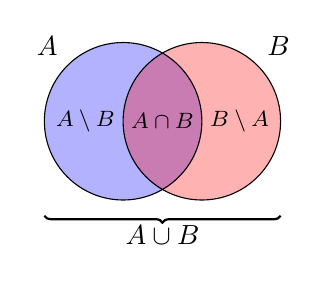
\begin{tikzpicture}
                        \node [above left] at (135:1) {$A$};
                        \node [above right] at ([xshift=1cm]45:1) {$B$};
                        \draw [thick,decorate,decoration={brace,mirror}] (-1,-1.2) -- node[below]{$A\cup B$} (2,-1.2);

                        \footnotesize
                        \fill [fill=blue,opacity=0.3] circle (1cm);
                        \fill [fill=red,opacity=0.3] (1,0) circle (1cm);
                        \draw circle (1cm) node[left]{$A\setminus B$};
                        \draw (1,0) circle (1cm) node[right]{$B\setminus A$};
                        \node at (0.5,0) {$A\cap B$};
                    \end{tikzpicture}
                    \caption{Set union Venn diagram.}
                    \label{fig:vennDiagram}
                \end{figure}
                \begin{proof}
                    All of these claims can be read directly from the above diagram --- for the sake of space and because proving these claims is not the main point of this exercise, a rigorous proof of this lemma will be omitted.
                \end{proof}
            \end{lemma*}
            Back to the main claim, we want to show that $|A\cup B|+|A\cap B|=|A|+|B|$, which we can do by using the above lemma to justify various manipulations inspired by part (b). To begin, use Lemma (a) as follows.
            \begin{align*}
                |A\cup B|+|A\cap B| &= |(B\setminus A)\cup A|+|A\cap B|
                \intertext{Since $(B\setminus A)\cup A$ is a union of two disjoint sets (see Lemma (b)), it follows by part (b) that the above}
                &= |B\setminus A|+|A|+|A\cap B|\\
                &= |A|+|B\setminus A|+|A\cap B|
                \intertext{Since $B\setminus A$ and $A\cap B$ are disjoint (see Lemma (d)), we know that the above}
                &= |A|+|(B\setminus A)\cup(A\cap B)|
                \intertext{Lastly, apply Lemma (c):}
                &= |A|+|B|
            \end{align*}
        \end{proof}
        \item \marginnote{10/13:}$|A\times B|=|A|\cdot|B|$.
        \begin{proof}
            Let $|A|=n$ and $|B|=m$. Then since $A$ and $B$ are finite, Definition \ref{dfn:1.30} and \ref{dfn:1.28} tell us that there exist bijections $f:A\to[n]$ and $g:B\to[m]$. By Definition \ref{dfn:1.33} and \ref{dfn:1.28}, to prove the claim, it will suffice to find a bijection $h:A\times B\to[m\cdot n]$.\par
            Let $h:A\times B\to[m\cdot n]$ be defined by
            \begin{equation*}
                h(a,b) = f(a)+n\cdot(g(b)-1)
            \end{equation*}
            Clearly, the above rule assigns a unique value to every $(a,b)$, and since $f$ and $g$ map all $a\in A$ and $b\in B$, respectively, the above function is not undefined for any $(a,b)\in A\times B$. Thus, $h$ is a function as defined in Definition \ref{dfn:1.16}.\par
            We must now prove that $h$ is bijective. By Definition \ref{dfn:1.20}, it will suffice to prove that $h$ is injective and surjective, which we may do as follows. We shall start with injectivity.\par
            Let
            \begin{align*}
                h(a,b) &= h(a',b')
                \intertext{Then by the definition of $h$,}
                f(a)+n\cdot(g(b)-1) &= f(a')+n\cdot(g(b')-1)\\
                f(a)-f(a') &= n\cdot(g(b')-1)-n\cdot(g(b)-1)\\
                f(a)-f(a') &= n\cdot(g(b')-g(b))
            \end{align*}
            Since $f(a)$ and $f(a')$ are both elements of $[n]$, we have $|f(a)-f(a')|<n$ (since $\max([n])-\min([n])=n-1<n$). Substituting, we have that $|n\cdot(g(b')-g(b))|<n$, i.e., $|g(b')-g(b)|<1$. But since $g(b),g(b')\in[m]$, the only way that $|g(b')-g(b)<1$ is if $|g(b')-g(b)|=0$. Consequently, $g(b')-g(b)=0$, so additionally, $f(a)-f(a')=n\cdot(g(b')-g(b))=0$. Having ascertained that $g(b')-g(b)=0$ and $f(a)-f(a')=0$, it is a simple matter to find that $g(b)=g(b')$ and $f(a)=f(a')$, meaning by the bijectivity (more specifically, the injectivity) of $f$ and $g$ that $b=b'$ and $a=a'$. But by Definition \ref{dfn:1.15}, this implies that $(a,b)=(a',b')$, as desired.\par
            As to surjectivity, let $c$ be an arbitrary element of $[n\cdot m]$. As a natural number, $c$ can be written in the form $c=\beta\cdot n+\alpha$ where $1\leq\alpha\leq n$ and $\beta\in\N$. We know that $\min([n\cdot m])=1=0\cdot n+1$ and $\max([n\cdot m])=m\cdot n=(m-1)\cdot n+n$; thus, if we restrict the possible values of $\beta$ to $0\leq\beta\leq m-1$, we still know that $c=\beta\cdot n+\alpha$ for some $1\leq\alpha\leq n$ and $0\leq\beta\leq m-1$. Now by the surjectivity of $f$, there exists an $a\in A$ such that $f(a)=\alpha$ for any $1\leq\alpha\leq n$. Similarly, the surjectivity of $g$ implies that there exists a $b\in B$ such that $g(b)=\beta+1$ for any $1\leq\beta+1\leq m$, i.e., there exists a $b\in B$ such that $g(b)-1=\beta$ for any $0\leq\beta\leq m-1$. Therefore, $c$ can be written in the form $c=f(a)+n\cdot(g(b)-1)$ for some $a\in A$ and $b\in B$, which by the definition of $h$ means that $c=h(a,b)$ for some $(a,b)\in A\times B$, as desired.
        \end{proof}
    \end{enumerate}
\end{exercise}

\begin{definition}\label{dfn:1.35}\marginnote{10/8:}
    An infinite set $A$ is said to be \textbf{countable} if it is in bijective correspondence with $\N$. An infinite set that is not countable is called \textbf{uncountable}.
\end{definition}

\begin{exercise}\label{exr:1.36}
    Prove that $\Z$ is a countable set.
    \begin{proof}
        To prove that $\Z$ is countable, Definition \ref{dfn:1.35} and, subsequently, Definition \ref{dfn:1.28} tell us that we must find a bijection $f:\Z\to\N$. To do so, we will define a matching and then prove that the guiding rule generates a (1) function that is (2) injective and (3) surjective (demonstrating injectivity and surjectivity verifies bijectivity by Definition \ref{dfn:1.20}).\par
        Let $f:\Z\to\N$ be defined as follows:
        \begin{equation*}
            f(z) =
            \begin{cases}
                -2z+1 & z\in-\N\\
                1 & z\in\{0\}\\
                2z & z\in\N
            \end{cases}
        \end{equation*}
        Since $\Z=(-\N)\cup\{0\}\cup(\N)$, it is clear that the above mapping sends every element of $\Z$ to \emph{an} element of $\N$. Additionally, since $-\N$, $\{0\}$, and $\N$ are all disjoint from one another, it follows that each element of $\Z$ is only mapped once. Thus, by Definition \ref{dfn:1.16}, $f$ is a function as defined.\par
        Let $f(z)=f(z')$. Since the outputs of the first case in the definition of $f$ are the odd natural numbers except 1, the one of the second case is 1, and those of the third case are the even natural numbers, the outputs form three disjoint sets, so $f(z)$ and $f(z')$ as equal quantities are elements of only one category. We now divide into three cases by category. First, suppose $f(z)=f(z')$ is an odd natural number not equal to 1. Then we have by the definition of $f$ that $-2z+1=-2z'+1$, implying by the cancellation laws of addition and multiplication, respectively, that $z=z'$. Second, suppose that $f(z)=f(z')=1$. Then $z=z'=0$ by the definition of $f$. Lastly, suppose $f(z)=f(z')$ is an even natural number. Then we have by the definition of $f$ that $2z=2z'$, implying by the cancellation law of multiplication that $z=z'$. Therefore, in any case, $f(z)=f(z')$ implies that $z=z'$, meaning by Definition \ref{dfn:1.20} that $f$ is injective.\par
        Let $n$ be an arbitrary element of $\N$. As noted in "What is a mathematical proof?", $n$ must be either odd or even. Now if $n$ is odd, $n$ is either equal to 1 or not equal to 1. Thus, we can break the natural numbers $\N$ into three disjoint sets: $\N=(\{n\in\N:n\text{ is odd}\}\setminus\{1\})\cup\{1\}\cup\{n\in\N:n\text{ is even}\}$. We now divide into three cases, each pertaining to one of the disjoint subsets of $\N$ defined above. First, suppose $n$ is odd and not equal to 1. Then $n=2z+1$ for some $z\in\N$ (see "What is a mathematical proof?"), or $-2z+1$ for some $z\in-\N$ (the negative signs cancel). By the definition of $f$, this $z\in-\N$ is the element of $\Z$ that $f$ sends to $n$. Second, suppose that $n=1$. Then since $f(0)=1$ by the definition of $f$, 0 is the element of $\Z$ from which $f$ generates 1. Lastly, suppose that $n$ is even. Then $n=2z$ for some $z\in\N$ (see "What is a mathematical proof?"). By the definition of $f$, this $z$ is the element of $\Z$ that $f$ sends to $n$. Therefore, for every element $n\in\N$, there exists a $z\in\Z$ satisfying $f(z)=n$, meaning by Definition \ref{dfn:1.20} that $f$ is surjective. As mentioned at the top, the last two results (injectivity and surjectivity) together imply that $f$ is bijective by Definition \ref{dfn:1.20}.
    \end{proof}
\end{exercise}

\begin{exercise}\label{exr:1.37}\marginnote{10/13:}
    Prove that every infinite subset of a countable set is also countable.
    \begin{lemma*}
        Every infinite subset of the natural numbers is countable.
        \begin{proof}
            Let $A\subset\N$ be infinite. To prove that $A$ is countable, Definition \ref{dfn:1.35} tells us that it will suffice to show that there exists a bijection $g:\N\to A$. Let's begin.\par
            We define $g$ recursively with strong induction, as follows. Note that $A=A\setminus\{\}$ where $\{\}=\emptyset$. By the well-ordering principle (see Script 0), there exists a minimum element $\min(A\setminus\{\})\in A\setminus\{\}$; we define $g(1)=\min(A\setminus\{\})$. Now suppose inductively that we have defined $g(1),g(2),\dots,g(n)$. Then we can define $g(n+1)$ by defining $g(n+1)=\min(A\setminus\{g(1),g(2),\dots,g(n)\})$\footnote{Basically, what this definition is doing is mapping 1 to the least element of $A$, 2 to the second-least element of $A$, 3 to the third-least element of $A$, and so on and so forth. Notice how the least element of $A$ is denoted by $g(1)$, and $g(2)$ (for example) is equal to $\min(A\setminus\{g(1)\})$, i.e., the minimum value in $A$ if $A$'s least element did not exist, i.e., the second-least element in $A$. Additionally, $g(3)=\min(A\setminus\{g(1),g(2)\})$, so we can see how $g(3)$ is the third-least element in $A$ by the same logic used in discussing $g(2)$. Obviously, the pattern continues for all $n\in\N$.}. By the principle of strong mathematical induction, it follows that $g$ is defined for all $n\in\N$, and it is obvious that $g$ is not multiply defined for any $n\in\N$. Thus, $g$ is a function as defined in Definition \ref{dfn:1.16}.\par
            To prove that $g$ is bijective, Definition \ref{dfn:1.20} tells us that it will suffice to show that $g$ is injective and surjective. We will prove each of these qualities in turn. To prove that $g$ is injective, Definition \ref{dfn:1.20} tells us that we must verify that $n\neq n'$ implies $g(n)\neq g(n')$. Suppose that $n\neq n'$. Then by the trichotomy, either $n>n'$ or $n<n'$. If $n>n'$, then $g(n)=\min(A\setminus\{g(1),\dots,g(n'),\dots,g(n-1)\})$, meaning that $g(n)$ cannot equal $g(n')$ since $g(n)$ is an element of a set (namely, $A\setminus\{g(1),\dots,g(n'),\dots,g(n-1)\}$) of which $g(n')$ is explicitly not a member. The proof is symmetric if $n<n'$. To prove that $g$ is surjective, Definition \ref{dfn:1.20} tells us that we must verify that for all $a\in A$, there exists an $n\in\N$ such that $g(n)=a$. Suppose for the sake of contradiction that there exists some $a\in A$ such that $g(n)\neq a$ for any $n\in\N$. This implies that $a\neq\min(A\setminus\{g(1),\dots,g(n)\})$ for any $n\in\N$, which must mean that $a\notin A$, a contradiction.
        \end{proof}
    \end{lemma*}
    \begin{proof}
        Let $A$ be a countable set and let $B\subset A$ be an infinite set. By Definition \ref{dfn:1.35} and \ref{dfn:1.28}, there exists a bijection $f:A\to\N$. Now consider the set $f(B)$. Clearly $\tilde{f}:B\to f(B)$ defined by $\tilde{f}(b)=f(b)$ is a function and a bijection. Since $f(B)\subset\N$ is infinite, there exists a bijection $g:f(B)\to\N$ by the lemma and Definition \ref{dfn:1.35}. It follows by Proposition \ref{prp:1.26} that $g\circ\tilde{f}:B\to\N$ is a bijection, proving that $B$ is countable by Definition \ref{dfn:1.35}, as desired.
    \end{proof}
\end{exercise}

\begin{exercise}\label{exr:1.38}
    Prove that if there is an injection $f:A\to B$ where $B$ is countable and $A$ is infinite, then $A$ is countable.
    \begin{proof}
        Let $\tilde{f}:A\to f(A)$ be defined by $\tilde{f}(a)=f(a)$. To prove that $\tilde{f}$ is a function, Definition \ref{dfn:1.16} tells us that it will suffice to show that for all $a\in A$, there exists a unique $b\in f(A)$ such that $\tilde{f}(a)=b$. Let $a$ be an arbitrary element of $A$. It follows by Definition \ref{dfn:1.18} that $f(a)\in f(A)$, hence $\tilde{f}(a)\in A$ by the definition of $\tilde{f}$. Furthermore, since $f(a)$ is a unique object, $\tilde{f}(a)$ is also a unique object.\par
        To prove that $\tilde{f}$ is bijective, Definition \ref{dfn:1.20} tells us that it will suffice to show that $\tilde{f}$ is injective and surjective. We will verify these two characteristics in turn. To prove that $\tilde{f}$ is injective, Definition \ref{dfn:1.20} tells us that we must demonstrate that $\tilde{f}(a)=\tilde{f}(a')$ implies $a=a'$. Let $\tilde{f}(a)=\tilde{f}(a')$. By the definition of $\tilde{f}$, $\tilde{f}(a)=f(a)$ and $\tilde{f}(a')=f(a')$. Thus, $f(a)=\tilde{f}(a)=\tilde{f}(a')=f(a')$, i.e., $f(a)=f(a')$. As such, by the injectivity of $f$, $a=a'$, as desired. To prove that $\tilde{f}$ is surjective, Definition \ref{dfn:1.20} tells us that we must demonstrate that for all $b\in f(A)$, there exists an $a\in A$ such that $\tilde{f}(a)=b$. Let $b$ be an arbitrary element of $f(A)$. By Definition \ref{dfn:1.18}, it follows that $b=f(a)$ for some $a\in A$. But by the definition of $\tilde{f}$, we also have $f(a)=\tilde{f}(a)$, so transitivity implies that $\tilde{f}(a)=b$, as desired.\par
        Since $A$ is infinite, Definition \ref{dfn:1.30} tells us that no bijection $h:A\to[n]$ exists for any $n\in\N$. Consequently, since there exists a bijection $\tilde{f}:A\to f(A)$, no bijection $h:f(A)\to[n]$ exists, implying by Definition \ref{dfn:1.30} that $f(A)$ is similarly infinite. In addition to being infinite, Definition \ref{dfn:1.18} asserts that $f(A)\subset B$. Thus, Exercise \ref{exr:1.37} applies and proves that $f(A)$ is countable. It follows by Definition \ref{dfn:1.35} that there exists a bijection $g:f(A)\to\N$. Since $\tilde{f}$ and $g$ are both bijective, Proposition \ref{prp:1.26} implies that $g\circ\tilde{f}:A\to\N$ is bijective. Therefore, $A$ and $\N$ are in bijective correspondence by Definition \ref{dfn:1.28}, meaning that $A$ is countable by Definition \ref{dfn:1.35}.
    \end{proof}
\end{exercise}

\begin{exercise}\label{exr:1.39}
    Prove that $\N\times\N$ is countable by considering the function $f:\N\times\N\to\N$ given by $f(n,m)=(10^n-1)10^m$.
    \begin{lemma*}[Informal\footnote{Dr. Cartee approved this.}]
        If $10^a+10^b=10^c+10^d$ for $a,b,c,d\in\N$, then either $a=c$ and $b=d$, or $a=d$ and $b=c$.
        \begin{figure}[h!]
            \centering
            \begin{subfigure}[b]{0.18\linewidth}
                \centering
                \begin{tikzpicture}
                    \footnotesize
                    \node{$100\cdots 00$};

                    \scriptsize
                    \node at (0,-1.1) {\textcolor{white}{$10^d$ causes this}};
                \end{tikzpicture}
                \caption{$10^a$.}
                \label{fig:base10a}
            \end{subfigure}
            \begin{subfigure}[b]{0.18\linewidth}
                \centering
                \begin{tikzpicture}
                    \footnotesize
                    \node{$100\cdots 010\cdots 00$};

                    \scriptsize
                    \node at (0,-1.1) {\textcolor{white}{$10^d$ causes this}};
                \end{tikzpicture}
                \caption{$10^a+10^b$.}
                \label{fig:base10b}
            \end{subfigure}
            \begin{subfigure}[b]{0.6\linewidth}
                \centering
                \begin{tikzpicture}
                    \footnotesize
                    \node{$100\cdots 010\cdots 00$};

                    \small
                    \node (cases) at (-5.5,0) {Two cases};
                    \node (1c) at (-2.5,-0.7) {$10^c$ causes this};
                    \node (1d) at (-2.5,-1.1) {$10^d$ causes this};
                    \node (2d) at (-2.5,0.7) {$10^d$ causes this};
                    \node (2c) at (-2.5,1.1) {$10^c$ causes this};

                    \begin{scope}[semithick,-stealth]
                        \draw (cases) to[out=0,in=180] ($(2c.west)!0.5!(2d.west)$);
                        \draw (cases) to[out=0,in=180] ($(1c.west)!0.5!(1d.west)$);

                        \draw (1c) to[out=0,in=-90] (-0.97,-0.2);
                        \draw (1d) to[out=0,in=-90] (0.07,-0.2);
                        \draw (2d) to[out=0,in=90] (-0.97,0.2);
                        \draw (2c) to[out=0,in=90] (0.07,0.2);
                    \end{scope}
                \end{tikzpicture}
                \caption{Possible matchings of $10^c$ and $10^d$.}
                \label{fig:base10c}
            \end{subfigure}
            \caption{Base-10 representations (ignoring the case where $a=b$).}
            \label{fig:base10}
        \end{figure}
        \begin{proof}
            Refer to Figure \ref{fig:base10} throughout the following discussion. Think about the base-10 representation of $10^a$ --- it will be a 1 followed by a bunch of 0s. When we add $10^b$ to $10^a$, either one of the 0s becomes a 1, the 1 becomes a 2, or a further string consisting of a 1 (possibly followed by 0s) is concatenated to the beginning of the existing number. In any of these cases, it is clear that for this number to be written in the form $10^c+10^d$, one of those two terms ($10^c$ or $10^d$) must account for one of the 1s, and the other for the other 1 (or both for the 2, in that case).
        \end{proof}
    \end{lemma*}
    \begin{proof}
        We wish to prove that $f$ is injective, so that Exercise \ref{exr:1.38} applies. By Definition \ref{dfn:1.20}, proving that $f$ is injective necessitates showing that $f(a,b)=f(c,d)$ implies that $(a,b)=(c,d)$ for all $(a,b),(c,d)\in\N\times\N$. Let $(a,b),(c,d)$ be arbitrary elements $\N\times\N$, and suppose that
        \begin{align*}
            f(a,b) &= f(c,d)
            \intertext{Substituting the definition of $f$ and algebraically manipulating, we get}
            (10^a-1)(10^b) &= (10^c-1)(10^d)\\
            10^{a+b}-10^b &= 10^{c+d}-10^d\\
            10^{a+b}+10^d &= 10^{c+d}+10^b
        \end{align*}
        By the lemma, either $a+b=b$ and $c+d=d$, or $a+b=c+d$ and $b=d$. In the first case, we must have $a=0$ and $c=0$ for the equalities to hold. But since $0\notin\N$, this implies that $a,c\notin\N$, a contradiction. Thus this case does not hold and it must be that the second case is true. In the second case, $b=d$, so by the cancellation law for addition, $a=c$. Since $a=c$ and $b=d$, Definition \ref{dfn:1.15} tells us that $(a,b)=(c,d)$, as desired.\par
        Having proven that there exists an injection $f:\N\times\N\to\N$ where $\N$ is (clearly) countable and $\N\times\N$ is (clearly) infinite, Exercise \ref{exr:1.38} implies that $\N\times\N$ is countable, as desired.
    \end{proof}
\end{exercise}

\subsubsection*{Additional Exercises}
\begin{enumerate}
    \item \marginnote{10/6:}In each of the following, write out the elements of the sets.
    \begin{enumerate}
        \item[a)] $(\{n\in\Z\mid n\text{ is divisible by }2\}\cap\N)\cup\{-5\}$
        \begin{proof}
            The elements are $-5$ as well as 2, 4, 6, and every other even natural number.
        \end{proof}
        \item[c)] $\{[n]\mid n\in\N,1\leq n\leq 3\}$
        \begin{proof}
            The elements are the three sets $\{1\}$, $\{1,2\}$, and $\{1,2,3\}$.
        \end{proof}
        \item[k)] $\{\{a\}\cup\{b\}\mid a\in\N,b\in\N,1\leq a\leq 4,3\leq b\leq 5\}$
        \begin{proof}
            The elements are the 11 sets $\{1,3\}$, $\{1,4\}$, $\{1,5\}$, $\{2,3\}$, $\{2,4\}$, $\{2,5\}$, $\{3\}$, $\{3,4\}$, $\{3,5\}$, $\{4\}$, and $\{4,5\}$.
        \end{proof}
    \end{enumerate}
\end{enumerate}




\end{document}